\documentclass[11pt,a4paper,twoside,BCOR=1cm,DIV=11,headsepline]{scrreprt} %draft

%***************Start Paket-Einbindungen******************
\usepackage[latin1]{inputenc} %textcodierung, in windows auch latin1, in unix utf8
\usepackage[ngerman]{babel}		%deutsche Sprachtrennung
\usepackage{amsfonts,amsmath,amsthm}	
\usepackage{makeidx}	%fuer Verwendung des index'
\usepackage[colorlinks=false,pdfborder={0 0 0},plainpages=false]{hyperref} %fuer hyperlinks im pdf-format
%GENAU DANN verwenden, wenn digital veroeffentlicht
%\usepackage{sidecap} % um \caption{?} neben bildern m�glich zu machen
\usepackage{pgf} %fuer grafiken
\usepackage{here}
\usepackage{graphicx}

% Glossar
%\usepackage{glossaries}
%***************Ende Paket-Einbindungen******************

%**************Start Allgemeine Optionen*****************
\setkomafont{sectioning}{\rmfamily\bfseries\boldmath}
\makeindex
%\hyphenation{geo-d�-tisch Geo-d�-te L�n-gen-raum un-ter-halb-ste-tig un-ter-halb-ste-ti-ge Ver-gleichs-drei-ecke Alex-an-drov} %hier geh�ren zu trennende W�rter hin, die Latex nicht kennt
%% Gleichungen nach Kapitel nummerieren
\renewcommand{\theequation}{\thechapter.\arabic{equation}}
\numberwithin{equation}{chapter}
%\setlength{\parindent}{0pt} %kein Einzug (nie)
%\addtolength{\leftmargini}{2.5em}
%****************Ende Allgemeine Optionen*************

%************** Start Befehle *************
%Aenderung der Nummerierungsart (klein roemisch)
\renewcommand{\labelenumi}{(\roman{enumi})}
%************** Ende Befehle **************


%************** Start Grafik **********
\providecommand{\graphic}[1]{\begin{center}{\footnotesize \input{graphics/#1.TpX}}\end{center}}
%************** Ende Grafik *********** 			%hier sind alle wichtigen eigenschaften 
											%des Dokuments vorgelegt
\begin{document}
\pagestyle{empty}
\pagenumbering{alph}
\begin{titlepage}
%\mbox{}

\vspace{0.1\textheight}

\begin{center}
{\sc\Huge Content�bergabe an eine Mobile App �ber ein CMS\\}

\vspace{0.1\textheight}

Alexander Gustafson\\
Ramon Schilling\\
\today

\vspace{0.15\textheight}

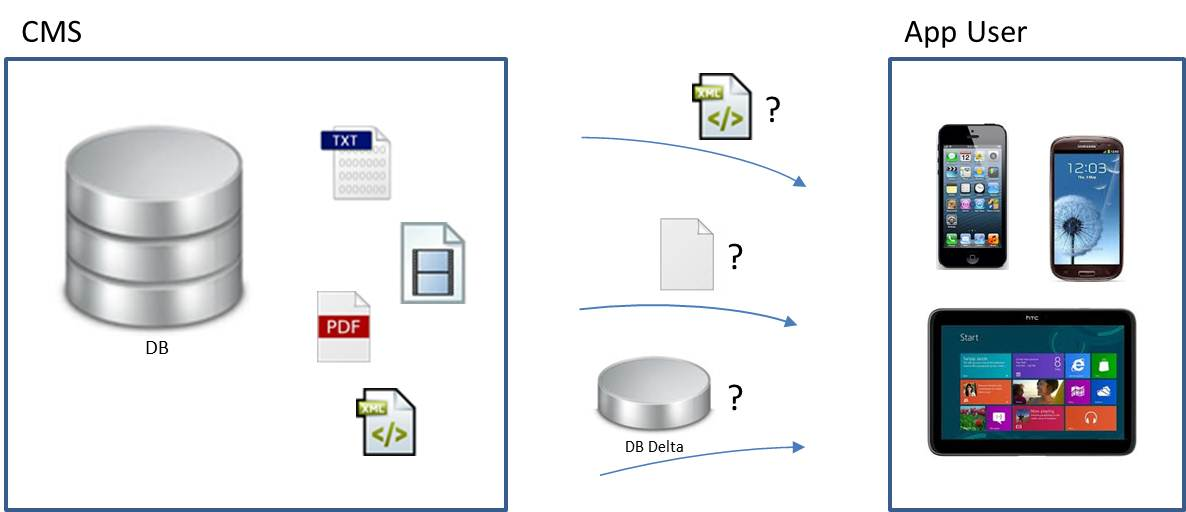
\includegraphics[width=0.70\textwidth]{graphics/titelbild.jpg}



\vspace{0.15\textheight}

Seminararbeit\\
ausgef�hrt an der\\ \vspace{0.3 cm}
Z�rcher Hochschule f�r Angewandte Wissenschaften (ZHAW)\\
Studiengang Informatik\\ \vspace{0.3 cm}
im Seminar "Handheld"\\ \vspace{0.3 cm}
unter der Leitung von\\
Christian Vils
\end{center}
\end{titlepage}

\cleardoublepage
\pagenumbering{roman}   % i, ii, iii, iv, ...
\setcounter{page}{1}
\cleardoublepage
\tableofcontents			%Inhaltsverzeichnis
\cleardoublepage
\cleardoublepage
\pagestyle{headings}
\pagenumbering{arabic}  % 1, 2, 3, 4, ...
\setcounter{page}{1}
\chapter{Einleitung}


\section{Ausgangslage}
F�r content-basierte Mobile Apps m�ssen immer wieder neue Inhalte publiziert werden. Dies soll jeweils vom Betreiber der App auf einfache Art m�glich sein. Dies ist m�glich, wenn die Inhalte in einem CMS verwaltet werden. Die App soll automatisch aktuell gehalten werden, ohne dass die ganze App aktualisiert werden muss, und auch ohne dass der Konsument aktiv wird. Wichtig ist zudem, dass die Daten auch offline zur Verf�gung stehen und auch gr�ssere Datenmengen unproblematisch �bermittelt werden k�nnen. Trotzdem muss aber ein Mechanismus gefunden werden, dass nur m�glichst kleine Datenmengen �bermittelt werden m�ssen um z.B. auf geringe Bandbreite reagieren zu k�nnen, oder Roaming-Geb�hren klein zu halten. Zum Beispiel m�ssen Apps von Museen, Ausstellungen, Konzertbetreibern oder Zeitschriften diese Anforderungen erf�llen

\section{Aufgabenstellung}
\begin{itemize}
\item Recherchieren, welche Produkte zur L�sung des Problems bereits bestehen und allf�llige Vor- und Nachteile dieser aufzeigen.
\item Aufzeigen welche L�sungsvarianten m�glich sind.
\item Einarbeiten in die Handheld Programmierung.
\item Auswahl von Techniken f�r die eigene Implementation.
\end{itemize}

\section{Zielsetzung}
Das Ziel der Seminararbeit ist es aufzuzeigen, welche Systeme, Prozesse und Design-Patterns wichtig sind und in Frage kommen um den oben genannten Anforderungen gerecht zu werden. Insbesondere die Schwierigkeit, m�glichst effizient aktuelle Daten dem App-Benutzer zur Verf�gung zu stellen soll dabei beachtet werden.

Falls m�glich k�nnen bereits gewisse Teile praktisch umgesetzt werden: z.B. kann ein CMS bereitgestellt werden, �ber welches der Betreiber der App die Inhalte bereitstellen und zur Aktualisierung f�r die App freigeben kann. Weiter kann eine App entwickelt werden, welche ihre Inhalte �ber das CMS bezieht und die definierten Prozesse umsetzt.


\section{Motivation}
Eine eigene Mobile App zu haben, ist heute f�r eine Firma oder eine Organisation fast schon so selbstverst�ndlich wie eine Website zu besitzen. Durch diese rasante Verbreitung von Mobile Apps wird es immer wichtiger, dass diese auch einfach aktuell gehalten werden k�nnen. Uns hat die Idee dieser Semesterarbeit deshalb fasziniert. 

Unabh�ngig von dieser Arbeit haben wir auch Anfragen aus dem Freundes- und Bekanntenkreis erhalten, welche sich f�r eine App interessierten, die f�r Promotionszwecke genutzt werden kann. Sie wollten wissen mit wie viel Aufwand eine solche App verbunden w�re. Da wir selbst keine Erfahrung in diesem Bereich hatten konnten wir auch keine Informationen geben. Dies hat uns aber zus�tzlich motiviert, nach geeigneten L�sungen zu suchen um die Erstellung von Apps, und vor allem die Erneuerung der Inhalte zu verinfachen.




\chapter{Projektmanagement}

\section{Projektteam}
Das Projektteam besteht aus Alex Gustafson und Ramon Schilling. Die Recherchearbeit haben wir zwischen beiden Projektmitgliedern aufgeteilt und die Resultat jeweils miteinander besprochen. Die Implementation wurde haupts�chlich von Alex Gustafson gemacht, w�hrend die Dokumentation von Ramon Schilling erstellt wurde.

\section{Termine}
\begin{tabbing}
12. Sept. 2012	\= -	\= Kick Off Meeting	\\
26. Sept. 2012	\> -	\> Abgabe der Aufgabe \\
28. Nov. 2012	\> -	\> Abgabe Teaser	\\
05. Dez. 2012	\> -	\> Arbeitstreffen	\\
13. Feb. 2013	\> -	\> Abgabe Schriftliche Arbeit	\\
20. Feb. 2013	\> -	\> Pr�sentation	\\
\end{tabbing}

\section{Projektplanung}

\section{Aufwand}
Der Aufwand f�r die Seminararbeit sollte pro Person 75 h betragen. Da wir die Arbeit zu zweit machen, haben wir unsere Planung deshalb auf 150 h ausgelegt. \\

\begin{tabular}{|l|c|c|}
\hline 
\textbf{Beschreibung} & \textbf{Soll}& \textbf{Ist} \\ 
\hline 
Recherche von m�glichen Synchronisationsabl�ufen & 30 h & 30 h \\ 
\hline 
Recherche bereits erh�lticher L�sungen & 10 h & 9 h \\ 
\hline 
Testen verschiedener Synchronisationsabl�ufe & 8 h & 12 h \\ 
\hline 
Einrichten der Entwicklungsumgebung & 4 h & 5 h \\ 
\hline
Programmieren / Testen CMS & 35 h & 40 h \\ 
\hline 
Programmieren iPhone App & 42 h & 38 h \\
\hline
Beispiel App erstellen & 12 h & 10 h \\
%Beispiel App Definition Thema, Umfang & 2 h & 2 h \\
\hline
%Beispiel App Templates definieren, erstellen & 4 h & 4 h \\ 
%\hline 
%Beispiel App Daten erstellen, eintragen & 4 h & 4 h \\
%\hline
Dokumentation & 13 h & 14 h \\ 
\hline 
\textbf{Total} & \textbf{154 h} & \textbf{158 h} \\
\hline
\end{tabular} 


\section{Hilfsmittel}

\subsection{Versionskontrolle}
Um eine Versionskontrolle zu haben, und damit wir beide gleichzeitig am Projekt arbeiten konnten, haben wir bei Github \cite{Github} ein Repository erstellt und s�mtliche f�r das Projekt n�tigen Dateien dort eingecheckt.

\subsection{Dokumentation}
Dokumentation haben wir mit \LaTeX{} erstellt.

\subsection{Programmierung}
Als Entwicklungsumgebung f�r die Programmierung mit PHP \cite{php} hat uns PHP Storm \cite{PhpStorm} gedient.
\newline
\\F�r die iPhone App Programmierung haben wir Xcode 4 \cite{Xcode} genutzt.
\newline
\\Als Datenbank haben wir auf SQLite \cite{sqlite} zur�ckgegriffen.
\newline
\\Das Optimus Dashboard \cite{optimus} nutzen wir bei der Entwicklung des CMS.
\newline
\\F�r den File Upload nutzten wir elfinder \cite{elfinder}.
\chapter{Recherche}

\section{Content Deployment}
Es gibt diverse Ans�tze um einer App den aktuellen Content zu �bergeben. Hier sollen verschiedene M�glichkeiten aufgezeigt und deren Vor- bzw. Nachteile kurz erl�utert werden.

\subsection{Ganze App aktualisieren}
Eine M�glichkeit ist selbstverst�ndlich bei jeder �nderung des Inhalts die gesamte App zu aktualisieren. Bei Apps mit statischem Inhalt welcher sehr selten wechselt kann das durchaus ein gangbarer Weg sein. Hat die App aber einen gr�sseren Umfang und werden regelm�ssig Inhalte ge�ndert ist diese Methode nicht geeignet da viele Anwender keine automatische Aktualisierung ihrer Apps zulassen und jedem Update zustimmen m�ssen.

\subsection{Web Application}
Bei einer Web Application wird der Inhalt jedes Mal wenn die App genutzt wird neu geladen. Grunds�tzlich handelt es sich um eine Website welche f�r die verschiedenen Ger�te angepasst wird. Der Vorteil dieser Methode besteht in der relativ einfachen Umsetzung. Damit die App genutzt werden kann, muss eine Internetverbindung bestehen. Dies ist nat�rlich ein Nachteil, da dies nicht immer gew�hrleistet werden kann und insbesondere im Ausland hohe Roaminggeb�hren anfallen k�nnen.

\subsection{Nur Daten aktualisiern}
Um eine App mit den m�glichst aktuellen Daten auch offline nutzen zu k�nnen, muss sich die App jeweils die neuen Daten herunterladen wenn eine Netzwerkverbindung zur Verf�gung steht. Der Vorteil ist nat�rlich, dass bei Inhaltsaktualisierungen nicht die ganze App aktualisiert werden muss und die App offline genutzt werden kann. Daf�r muss in der App zus�tzliche Logik eingebaut werden. Es muss jeweils �berpr�ft werden ob aktuellere Daten verf�gbar sind und diese m�ssen dann bei Bedarf und M�glichkeit heruntergeladen und �berpr�ft werden. Besonders bei grossen Datenbest�nden lohnt es sich, wenn nur �nderungen und nicht der gesamte Datenbestand �bermittelt wird.



\section{Marktsituation}
Wir haben uns mit der Frage besch�ftigt, welche Produkte es bereits gibt um einer App die Daten �ber ein CMS zur Verf�gung zu stellen.

Uns sind einige  interessante Produkte aufgefallen, welche die Plattformunabh�ngige Entwicklung von Apps erleichtern sollen und die Verteilung auf den verschiedenen Systemen vereinfachen. Dies geht zum Teil so weit, dass die aktualisierten Apps automatisch in den verschiedenen App Stores eingespielt werden und dass die Aktualisierung der bereits installieretn Apps automatisch �berwacht wird.

Weiter gibt es eine Menge an Produkten welche die Entwicklung von Web Applications erleichtern sollen.

Wir sind aber auf kein k�ufliches oder freies Produkt gestossen, welches sich auf die effizeinte Verteilung von Inhalten auf eine App spezialisiert. Es gibt zwar diverse Firmen welche Apps entwickeln und dem App-Betreiber erm�glichen Content �ber ein CMS zu verwalten. Da diese Firmen aber inhouse L�sungen benutzen, hatten wir keinen Einblick in die Art und Weise wie sie die Daten �bermitteln. 


\section{Datenspeicherung}
Die Form der Datenspeicherung hat Einfluss auf die M�glichkeiten wie die Daten verwaltet und �bermittelt werden k�nnen.

XML Files w�ren eine M�glichkeit, Daten textbasiert zu speichern. Da wir die M�glichkeit in Betracht ziehen die Daten �ber github zu verwalten, k�nnte diese Form der Datenspeicherung sehr n�tzlich sein. Ein Vorteil von dieser Variante w�re ausserdem, dass einzelne Dateien �bermittelt werden k�nnen.

Die Speicherung der Daten in einer relationalen Datenbank h�tte den Vorteil, dass durch die bin�re Speicherung weniger Speicherplatz ben�tigt wird und der Zugriff grunds�tzlich etwas schneller ist. Da dies aber vor allem bei grossen Datenmengen zum tragen kommt, ist dies kein ausschlaggebendes Kriterium. Mit SQLite existiert ausserdem eine Datenbank welche von allen g�ngigen Smartphone Systemen gut unterst�tzt wird.


\section{Verfahren f�r die Daten�bermittlung}
Unser Ziel ist es eine Umgebung zu entwicklen, in welcher eine Appe mit aktuellen Inhalten versorgt wird, die Inhalte aber auch offline Nutzen kann. 

\subsection{�nderungen �bermittlung}
Um auch bei h�ufigen �nderungen das zu �bertragende Datenvolumen m�glichst klein zu halten ist es wichtig, dass nicht bei jeder �nderung s�mtliche Daten �bertragen werden. Es sollen jeweils nur die ge�nderten Daten �bermittelt werden.

\subsection{git}
Versionierungssysteme wie z.B. git \cite{git} setzen diese Technik um. Wir haben deshalb die M�glichkeit gepr�ft, die Daten�bermittlung vom CMS zur Mobile App �ber github zu l�sen. Ein Vorteil bei diesem Vorgehen w�re, dass die Logik zur Ermittlung der �nderungen nicht neu entwickelt werden m�sste. Da git zwar �nderungen in Bin�rdateien erkennt, aber nur bei Text-Dateien die Differenz markieren kann, kommt der Vorteil von git nur bei Text-Dateien zum Tragen. Dieses Verfahren w�rde deshalb die Auswahl des Datenformats beeinflussen. Ausserdem gibt es zwar f�r alle g�ngigen Smartphone Systeme git-Clients, diese haben aber nicht alle Funktionen von git implmentiert.\\
\\
Der entscheidende Punkt welcher gegen den Einsatz von github sprach, liegt aber bei der Art und Weise wie github funktioniert. �nderungen welche auf github gepusht (heraufgeladen) werden, werden dort nur akzeptiert, wenn der Client zuvor die aktuellste Version gepullt (heruntergeladen) hatte und einen Merge (eine Art Synchronisation der Datenbest�nde) gemacht hatte. Das gibt dem Client die M�glichkeit nur die �nderungen zu pushen, und nicht alle Daten. Werden im CMS Daten ge�ndert und dann auf github gepusht, werden also nur die �nderungen �bermittelt.

Fordert aber ein Client die aktuellen Daten an, macht er einen Pull und es wir ihm alles �bermittelt. Die Mobile App w�rde sich also immer alle Daten herunterladen. \\
\\
Es gibt die M�glichkeit, Patches zu erstellen, welche nur gewisse �nderungen enthalten. Diese Patches k�nnten dann zu den mobilen Endger�ten �bermittelt werden. Da nicht auf allen Endger�ten der selbe Stand der Daten vorhanden ist, m�ssten dies Patches verwaltet werden. Ausserdem unterst�tzen nicht alle freien git-Clients f�r Smartphone die Verwendung von Patches. \\
\\
Um mit github arbeiten zu k�nnen, m�sste also sowohl Serverseitig die Patchverwaltung, wie auch in der Mobile App gewisse git-Funktionalit�t und die Patchverarbeitung aufwendig implementiert werden. Da dies den Rahmen dieser Arbeit sprengen w�rde und nicht dem Fokus dieser Arbeit entspricht haben wir diese Idee verworfen. 

\subsection{Database Change Log Files}
S�mtliche �nderungen in einer Datenbank kann man in einem Log File speichern. Dazu werden alle ausgef�hrten SQL Statements welche �nderungen in der Datenbank zur Folge haben in dieses Log File geschrieben. Erstellt man f�r jede Version der Datenbank ein eigenes solches Log File, kann man jede �ltere Version der Datenbank in eine neuere Version �berf�hren, indem man die entsprechenden SQL Statements sequentiell abarbeitet.

Im Einsatz mit einer Mobile App werden viele zus�tzliche Resourcen wie Bilder, Videos, usw. genutzt. Es m�sste also ebenfalls festgehalten werden, welche Resourcen hinzugef�gt wurden. Diese Resourcen k�nnen in einem seperaten Log File aufgelistet werden, welches ebenfall f�r jede Version der Datenbank erstellt wird.\\
\\
Anstatt die gesamte Datenbank und s�mtliche Resourcen zu �bermitteln, m�sste der Mobile App anhand dieser beiden Log Files nur die neuen Resourcen und die n�tigen SQL Statements mit den Datenbank�nderungen �bermittelt werden. 

Um auf dem mobilen Endger�t Platz zu sparen, empfiehlt es sich nicht mehr gebrauchte Resourcen zu l�schen. Um dies zu bewerkstelligen kann die mobile App ihren Datenbestand nach nicht mehr gebrauchten Resourcen durchsuchen, oder es wird mit dem Update eine Liste mitgegeben welche die zu l�schenden Resourcen enth�lt.



\chapter{Implementation}

\section{Aufbau}
Die Implementation besteht aus einem CMS in welchem der Content von einer oder mehreren Apps verwaltet werden kann. Die Inhalte werden in einer Datenbank gespeichert. Eine iPhone App kann sich dann die Inhalte aus der Datenbank herunterladen und darstellen, bzw. verarbeiten.

\section{Datenstruktur}
Um eine gr�sstm�gliche Flexibilit�t zu gew�hrleisten wird die Datenstruktur nicht vorgeschrieben, sondern kann den Bed�rfnissen angepasst erstellt werden.

\begin{figure}[H]
	\centering
	\includegraphics[scale=0.8]{graphics/entityModel.png}
	\caption{\textbf{Entity Model} }
	\label{entityModel}
\end{figure}

In \autoref{entityModel} ist das Entit�tenmodell zu sehen auf welchem die Datenbank beruht. 

\subsection{Field\_types}
\emph{field\_types} k�nnen beliebig defniert werden. Es kann sich dabei um ein Attribut handeln, welches einen Status beschreiben soll, oder um eine Beschreibung eines Elements. Typische \emph{field\_types} sind z.B: text, url, color. Wichtig ist, dass ein \emph{field\_type} nicht einem Datentyp entsprechen muss. \\


\subsection{Templates}
Die \emph{Templates} sind das Herzst�ck der Datenstruktur. Es handelt sich dabei um eine Art Schablone, welche die Struktur f�r ein beliebiges Element vorgibt. Ein \emph{Template} kann entweder aus beliebig vielen \emph{Field\_types} bestehen (einfaches Template) oder aus beliebig vielen anderen \emph{Templates} und \emph{Field\_types} (Composite Template). \\
\\
Als Beispiel daf�r kann man sich ein Buch vorstellen, welches aus einem Titel und mehreren Kapiteln besteht. Titel und Kapitel w�ren \emph{Templates} welche aus dem \emph{Template} text bestehen und das \emph{Template} Buch w�rde aus den \emph{Templates} Titel und Kapitel bestehen.

\subsection{Articles}
Jeder \emph{Article} beruht auf einem \emph{Template}. Ein \emph{Article} ist die Umsetzung eines \emph{Templates} und entspricht einer dargestellten Seite in der App. Das \emph{Template} gibt die Struktur vor und die Daten werden entsprechend dieser Vorgabe als json-String abgelegt.

Die Mobile App interpretiert dann diesen json-String anhand der durch das Template vorgegebenen Struktur und stellt die Seite dar.

\section{Datenbank}
Als Datenbank haben wir uns f�r SQLite entschieden, da diese von allen verbreiteten Smartphone Systemen sehr gut unterst�tzt wird. \\
\\
Um die oben beschriebene Struktur in einer relationalen Datenbank abzubilden wird die Datenbank wie folgt aufgebaut:

\begin{figure}[H]
	\centering
	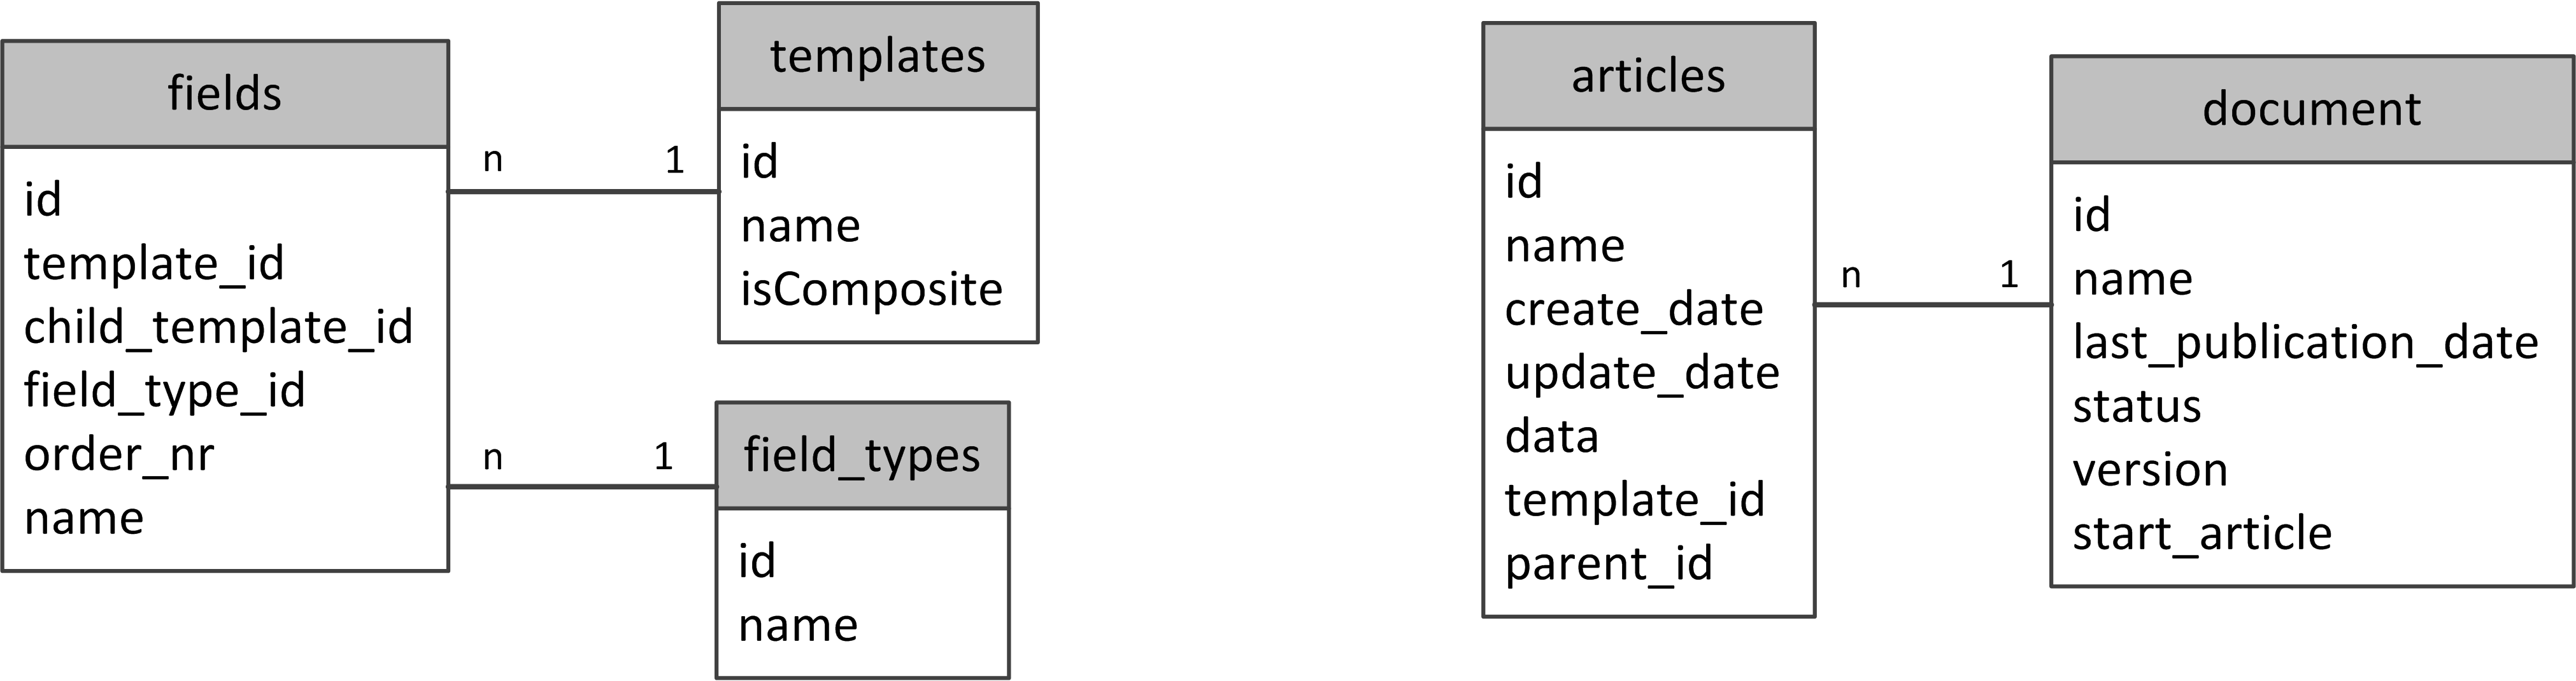
\includegraphics[scale=0.8]{graphics/db.png}
	\caption{\textbf{Database Model} }
	\label{dbModel}
\end{figure}

Die Zwischentabelle \emph{fields} wird ben�tigt um die Verschachtelung der \emph{Templates} und \emph{Field\_Types} zu erm�glichen. Jeder \emph{Article} ist einem  \emph{document} zugeordnet. Im \emph{document} wird der Start Artikel, Status und die Version der Daten festgehalten. Werden mehrere Apps in einer Datenbank verwaltet werden mehrere \emph{documents} erstellt.


\section{CMS}
Das CMS haben wir mit PHP entwickelt. Um die Benutzeroberfl�che schneller und benutzerfreundlicher gestalten zu k�nnen haben wir das Framework Optimus Dashboard genutzt. Das CMS ist in die Bereiche Dashboard, Documents, Articles, Templates und Assets unterteilt.

\subsection{Dashboard}
Dieser Bereich wird noch nicht gebraucht. Das Ziel ist es hier generelle Informationen anzuzeigen

\subsection{Documents}
Hier werden einzelne Documents (Apps) erstellt und verwaltet. Es kann der Startartikel f�r die App angegeben werden sowie die Version der Daten und der Status der App angepasst werden.

\subsection{Articles}
Dies ist der wichtigste Teil f�r die Bereitstellung von Inhalten. Hier werden die Artikel (Seiten der App) erstellt und bearbeitet. 

Um die Daten m�glichst einfach einzugeben, muss das CMS pro \emph{field\_type} eine ensprechende Eingabemaske anbieten (f�r \emph{text} ein Textfeld, f�r \emph{color} ein Color Picker, etc.).


\subsection{Templates}
Die f�r die Einrichtung wichtigen Templates k�nnen hier zusammengestellt werden. Dazu erlaubt das CMS die ben�tigten Felder zu verkn�pfen und zu gruppieren.

\subsection{Assets}
S�mtliche Resourcen wie Bilder, Videos, etc. k�nnen hier verwaltet werden.

\section{App}
Das Ziel ist, dass die App generisch ist, und grunds�tzlich keine Styles oder Bilder enth�lt. Jedes im CMS vorhandene Template sollte verarbeitet werden k�nnen. Dazu muss f�r iOS ein View Controller und f�r Android eine Activity implementiert sein. Bei anderen Systemen muss ebenfalls die Logik implementiert werden dass die m�glichen Templates verarbeitet und dargestellt werden. Je mehr Templates definiert sind und von der App unterst�tzt werden, desto mehr M�glichkeiten bieten sich an.

\subsection{Auf neue Inhalte �berpr�fen}

\begin{figure}[H]
	\centering
	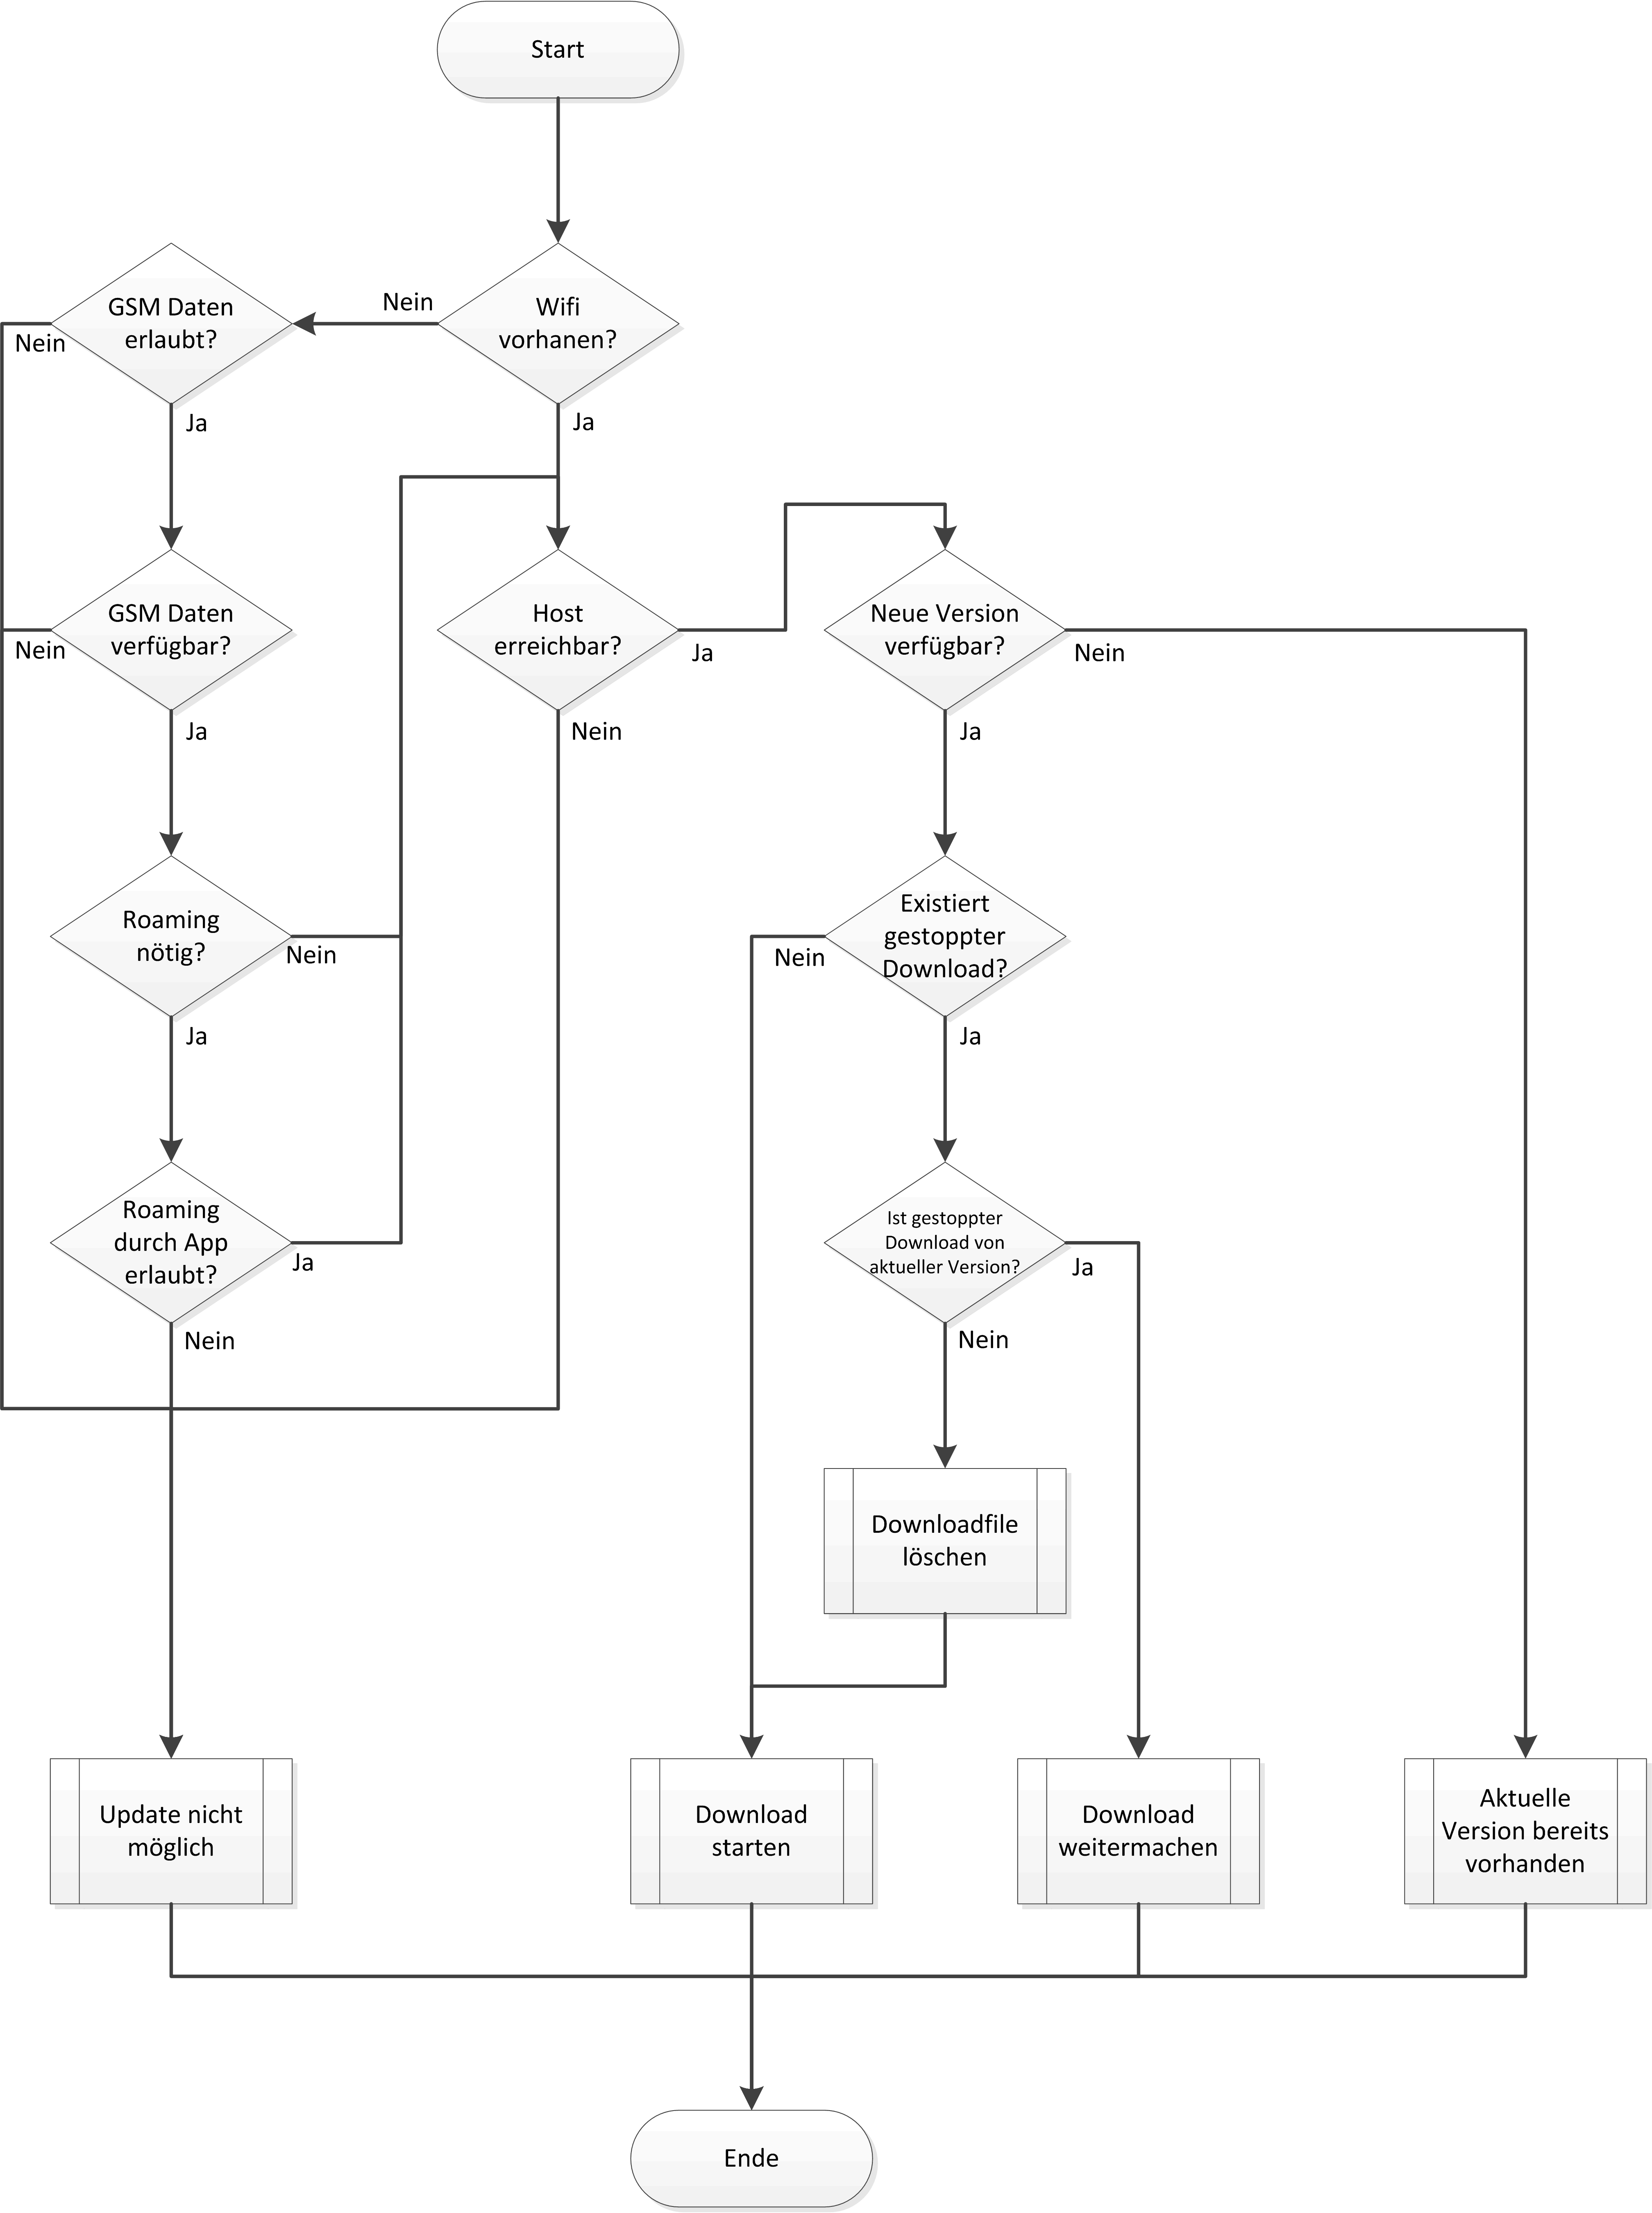
\includegraphics[scale=0.6]{graphics/Netzwerk-Check-FlowChart.png}
	\caption{\textbf{Ablaufdiagramm - Daten Update} }
	\label{NWCheck}
\end{figure}

\autoref{NWCheck} zeigt das Vorgehen der App zur Pr�fung ob neue Daten vorhanden sind. Wichtig ist die �berpr�fung ob Wifi vorhanden ist, bzw ob GSM Daten erlaubt sind. GSM steht hier stellvertretend f�r alle Mobiltelefonnetze. Da eine Datenverbindung �ber ein Mobiltelefonnetz mit Kosten verbunden sein kann (speziell Roaming-Geb�hren), fragt die App in diesem Fall nach, ob eine Verbindung gemacht werden darf. \\

\subsection{Interpretation von Artikeln}
Um ein Artikel darzustellen, analysiert die App den json-String, welcher im Datenfeld des Artikels hinterlegt ist. Anhand des Templates weiss die App wie der json-String zerlegt werden muss und die entsprechenden Elemente darzustellen sind.

\begin{figure}[H]
	\centering
	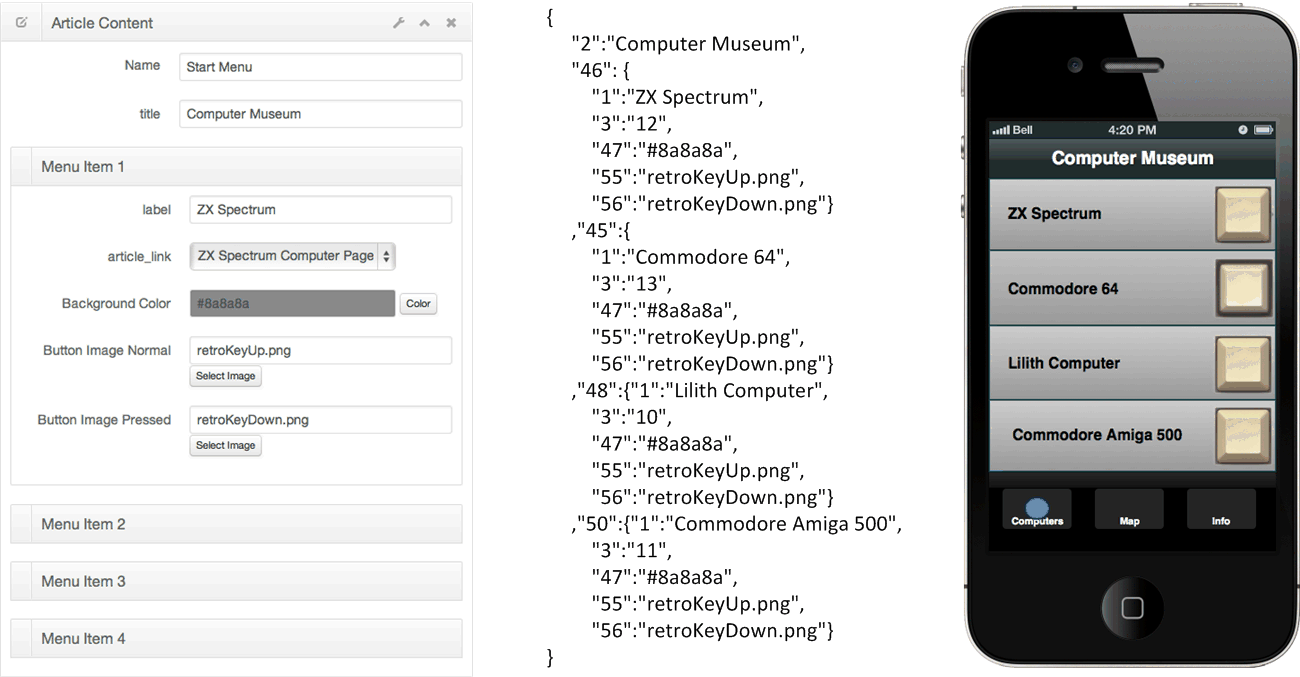
\includegraphics[scale=0.6]{graphics/jsonBsp.png}
	\caption{\textbf{Interpretation des json-Sting}}
	\label{jsonBsp}
\end{figure}

In \autoref{jsonBsp} sehen wir die schematische Darstellung des Templates im CMS, den json-String welcher das Template umsetzt und die Darstellung in der App.

\input{kap_beispielapp}
\chapter{Fazit}

In dieser Arbeit haben wir uns mit verschiedenen Fragestellungen befasst und nach neuen L�sungsans�tzen gesucht um auf einfache und effiziente Weise Inhalte f�r eine Mobiel App bereitzustellen und zu �bermitteln.

Wir hatten grosse Schwierigkeiten herauszufinden, welche Technologien und Verfahren bereits eingesetzt werden, da wir kein Produkt gefunden haben, welches sich prim�r mit der effizienten �bermittlung von Inhalten auf eine Mobile App befasst. Zus�tzlich sind fast keine technischen Informationen verf�gbar von Dienstleistern welche sich auf Mobile Apps spezialisiert haben. Das hat die Recherchearbeit erschwert und stellenweise auch etwas langatmig gemacht.

Trotzdem war die Aufgabe sehr spannend. Neben der Informationsbeschaffung und der Auseinandersetzung mit verschiedenen Technologien, haben wir ein eigenes CMS aufbauen k�nnen und eine App entwickelt, welche sich �ber dieses CMS aktualisieren l�sst. Das CMS und die App sind so aufgebaut, dass sich leicht neue Inhaltstypen und weitere Funktionalit�t implementieren l�sst.

Selbstverst�ndlich gibt es f�r die Zukunft noch viel Erweiterungspotential um welches wir uns im Rahmen dieser Arbeit nicht k�mmern konnten. Das System ist zwar so aufgebaut, dass man das CMS f�r mehrere Mandanten einsetzen k�nnte, diese Funktionalit�t ist aber noch nicht implementiert. Ebenso fehlt noch eine Userverwaltung und andere Sicherheitsaspekte wurden auch noch nicht ber�cksichtigt. ausserdem ist das L�schen von nicht mehr ben�tigten Bildern und anderen Assets auf dem Smartphone ein weiterer wichtiger Punkt.







\clearpage{\pagestyle{empty}\cleardoublepage}

\listoffigures
\chapter*{Literatur}

\textbf{elfinder}, Last Checked 20130213, URL http://elfinder.org/ \\
\\
\textbf{git}, Last Checked 20130213, URL http://git-scm.com/ \\
\\
\textbf{Github}, Last Checked 20130213, URL https://github.com/ \\
\\
\textbf{optimus}, Last Checked 20130213, URL  https://wrapbootstrap.com/theme/optimus-dashboard-admin-template-WB0016FX5/ \\
\\
\textbf{php}, Last Checked 20130213, URL http://php.net/ \\
\\
\textbf{PhpStorm}, Last Checked 20130213, URL http://www.jetbrains.com/phpstorm/ \\
\\
\textbf{sqlite}, Last Checked 20130213, URL http://www.sqlite.org/ \\
\\
\textbf{Xcode}, Last Checked 20130213, URL https://developer.apple.com/technologies/tools/ \\
\\






%\printbibliography
%\bibliographystyle{alphadin} %oder plainnatDeutsch (alphadin geht nicht mit natbib)amsalpha
%\bibliography{literatur}
%\clearpage{\pagestyle{empty}\cleardoublepage}
%\printindex										%fuer den Index

\end{document}

